\chapter{Backend and Runtime}
\label{chapter:backend-and-runtime}

This chapter discusses the last component of the SableWasm compilation pipeline, the code generation backend and runtime support for generated shared libraries. Currently, SableWasm has only one backend based on the LLVM compiler infrastructure. However, in the future, one can easily extend the system by adding more backends that lowering SableWasm MIR into other intermediate representations. Another problem that appears when designing a backend is how SableWasm MIR entities map to native constructs. In SableWasm, we take an instance-based approach. The SableWasm runtime library will manage all entities in an instance object. The system will pass it to the generated native functions as the first argument, similar to `this' pointer in many C++ implementations. In the rest of the chapter, we will first go through the design of the instance object, followed by implementation of WebAssembly entities. Finally, we will discuss the code generation strategies used when lowering SableWasm MIR to LLVM intermediate representation and the interaction between generated shared libraries and the hosting language.

\section{Instance Layout}

\begin{figure}
    \begin{minipage}{.35\textwidth}
        \centering
        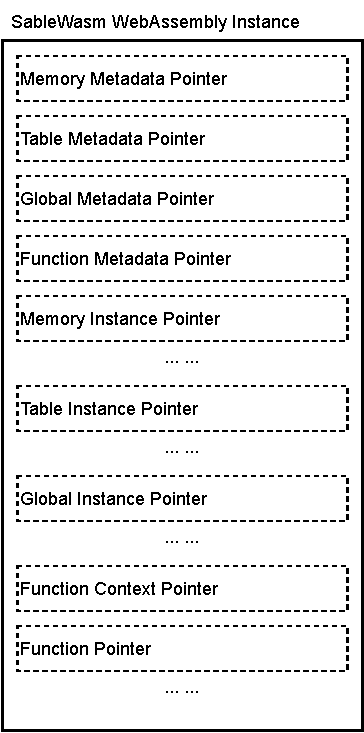
\includegraphics[width=\textwidth]{Images/5.Backend_and_Runtime/instance}
    \end{minipage}\hfill
    \begin{minipage}{.6\textwidth}
        \begin{lstlisting}[language=C, basicstyle=\ttfamily\footnotesize]
struct instance {
    memory_metadata_t   *memory_metadata;
    table_metadata_t    *table_metadata;
    global_metadata_t   *global_metadata;
    function_metadata_t *function_metadata;
    memory_t            *memories[NUM_MEMORY];
    table_t             *tables[NUM_TABLE];
    global_t            *globals[NUM_GLOBAL];
    struct {
        struct instance *context;
        function_t      *function_ptr;
    } * functions[NUM_FUNCTIONS];
};        
    \end{lstlisting}
    \end{minipage}
    \caption{SableWasm WebAssembly Instance}
    \label{fig:backend-instance}
\end{figure}

This section discusses the WebAssembly instance implementation in SableWasm. A WebAssembly instance hosts all the runtime structures that the generated shared libraries require, such as linear memory and indirect table. Figure~\ref{fig:backend-instance} illustrates the design of the WebAssembly instance. SableWasm's WebAssembly instance consists of two parts, metadata entries and entity pointers. One may also notice that the instance object's size may vary from modules to modules depending on how many entities are declared. This behaviour is intensional by design. SableWasm runtime system needs to compute the address of the pointers based on the metadata information on the fly. By packing all pointers in a consecutive memory region, we reduce one layer of indirection for the runtime system, and in theory, may improve runtime performance. On the other hand, the generated shared library has all the entities address inlined as the backend can infer them during code generation, which does not incur any performance loss. For most of the entities, they are pretty straightforward, and we will skip the discussion here. In the rest of the section, we focus on three aspects: the metadata entries, the function entity representations, and the instance initialization protocol in SableWasm.

\paragraph{Metadata}
One could think of the metadata as the signatures for entities, and indeed, the SableWasm runtime system prepares the instance object based on the metadata. Further, shared libraries generated by SableWasm only publicly expose the metadata and initialization function to conceal module details. Metadata encodes the type for the entity. For linear memories and indirect tables, this is relatively trivial as their types only consist of an integer pair. In the case of global values, things are a little bit complicated. A quick reminder, WebAssembly global types keep track of their value type and mutability. The first problem here is how to encode WebAssembly value types. One solution is to use WebAssembly value type binary format. However, this encoding strategy emits hard to maintain results as a human can not directly read them. Here we use the JVM approach for value type encoding \footnote{\url{https://docs.oracle.com/javase/7/docs/technotes/guides/jni/spec/types.html}}. A quick summary, in SableWasm, we encode 32-bit integers as `I', 64-bit integers as 'J', single-precision floating-point number as 'F', double-precision floating-point number as 'D' and finally, 128-bit vector type as 'V'. The second problem is how to encode global's mutability. In SableWasm, we use capital letters for constant global value types and lower letters for mutable ones. Finally, for function types, we follow a similar design as we used for global values. SableWasm encodes function type into a null-terminated string. Let's take \texttt{[i32, f32] -> [v128]} as an example. SableWasm encodes the type into `\texttt{IF:V}'. The colon acts as a separator between parameter types and result types. Note that `\texttt{:}' itself is also a valid SableWasm function type string, and represents \texttt{[] -> []}, a void function with no arguments. Finally, metadata also encode module names and entity names for import entities and names for export names, which play a critical role later in the module initialization phase.

\paragraph{Function entity representation}
WebAssembly specifications classify the functions into two groups, WebAssembly functions and host functions. WebAssembly functions are any functions defined within the module. On the other hand, the runtime system provides host functions to the module, and from the WebAssembly module point of view, the functions are black boxes without any knowledge of their internals. To make things more complex, although, in MVP WebAssembly, there are no explicit requirements on how the WebAssembly functions should behave if they are invoked from other modules. Here we use a similar generalization in Javascript \footnote{WebAssembly Javascript Interface: \url{https://www.w3.org/TR/wasm-js-api-1/}}. In summary, in SableWasm, if a module exports a function, it exports the function in a closure that captures its enclosing instance. Suppose a second module invokes the exported closure via import functions. In that case, the function still only has access to its original module's entities and only communicates with the second module via return values. Hence, in SableWasm, we implement our function as a pair of pointers. The first one refers to its enclosing instance, and the second one refers to pointers to the generated code. For host functions, we set the enclosing instance as a null pointer. In the chapter's introduction, we mentioned that we pass the instance object as the first argument to the generated functions. But, what should we pass to the host functions? SableWasm defines that for all the host functions, the instance object will always point to the caller's enclosing instance instead of null so that the host functions can access the internals of the caller's module.

\paragraph{Initialization protocol}
In the last part of the section, we will cover the initialization protocol we used in SableWasm. The initialization protocol consists of three basic steps, validation, instance preparation and initialization. In the validation phase, we load the shared library with the operating system's help, such as \texttt{dlopen} in Linux, and check if it contains all the required symbols. Currently, a SableWasm shared library needs to export five symbols in total. Table~\ref{table:sablewasm-runtime-export-syms} illustrates the symbols expected from the generated shared libraries. The instance initializer function takes a prepared instance object as the argument. The next step in SableWasm is to construct this prepared instance object. The idea of a prepared instance object is that we want to separate the memory allocation from the value initialization. In SableWasm, the runtime system handles the memory allocation, while on the other hand, the initializer function takes care of the value initialization. In the second phase, the SableWasm runtime allocates all the entities and attaches them to the module instance. Note that SableWasm also resolves all the import names at this stage, and it will only proceed to the next step if all the expecting import entities are set. Finally, the last step is the initialization. SableWasm will invoke the initializer function provided by the shared library. The initializer function takes care of all kinds of value initialization, such as setting values for global variables and copy data segments into linear memory.

\begin{table}[h]
    \centering
    \begin{tabular}{|l|l|}
        \hline
        \textbf{Symbol Name}          & \textbf{Description}         \\ \hline
        \_\_sable\_global\_metadata   & Metadata for global values   \\ \hline
        \_\_sable\_memory\_metadata   & Metadata for linear memories \\ \hline
        \_\_sable\_table\_metadata    & Metadata for indirect tables \\ \hline
        \_\_sable\_function\_metadata & Metadata for functions       \\ \hline
        \_\_sable\_initialize         & Instance initializer         \\ \hline
    \end{tabular}
    \caption{SableWasm shared libraries exported symbols}
    \label{table:sablewasm-runtime-export-syms}
\end{table}
\section{WebAssembly Entities}

In the previous section, we discuss the design of the SableWasm WebAssembly instance object. However, we treat all WebAssembly entities' implementation as an opaque pointer without diving into the details during the last section. This section will cover the implementation of the WebAssembly entities along with the runtime library support functions exposed to the generated code in SableWasm. Before we start this section, we will first present the terms used throughout the later part of the thesis. In the rest of the chapter, we use \texttt{\_\_sable\_instance\_t} to denote the type of the instance object. Similarly, we use a similar format when talking about WebAssembly linear memory, indirect table and global variables. For example, \texttt{\_\_sable\_instance\_t} is the type of SableWasm's WebAssembly linear memory implementation. Finally, we use \texttt{\_\_sable\_function\_t} refer to the function pointers that point to generated native functions.

\paragraph{Linear Memory}

\begin{figure}
    \centering
    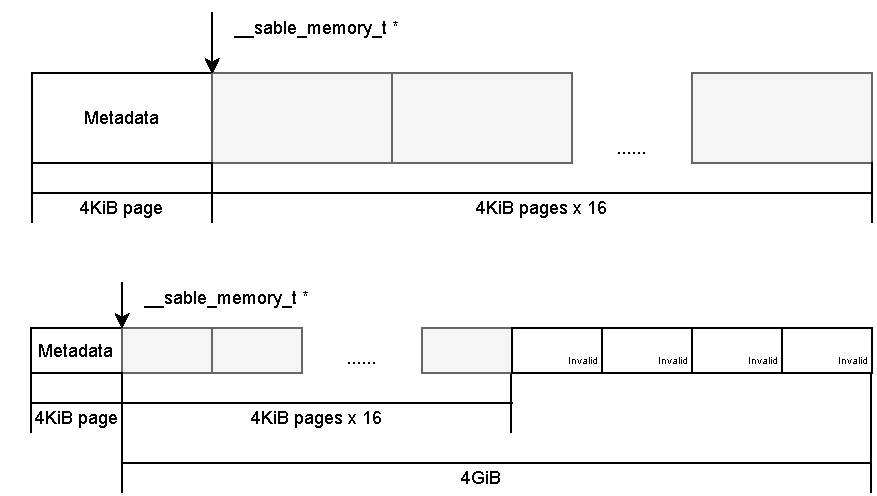
\includegraphics[width=0.85\textwidth]{Images/5.Backend_and_Runtime/memory}
    \caption{SableWasm WebAssembly linear memory}
    \label{fig:backend-memory}
\end{figure}

SableWasm implements WebAssembly linear memory with mapped memory provided by the operating system. It also has a fallback implementation that uses standard \texttt{malloc} and \texttt{free} procedure from the C library for an operating system that does not support mapped memory. The fallback implementation is relatively trivial, and we will not discuss it in the thesis. Here, we will focus on the one that uses mapped memory. Figure~\ref{fig:backend-memory} illustrates the strategies when mapping WebAssembly linear memory into native memory. On the top, we have a linear memory with a size of 1 in WebAssembly page size. In the figure, we assume the native machine has a page size of 4KiB, which is typical for most hardware architectures. A quick recap on the requirements of WebAssembly linear memory. First, the program can efficiently random access any location within the linear memory. Second, at runtime, the module function can query the size of the linear memory. Finally, the program can grow the linear memory if the runtime system allows it. SableWasm implements the linear memory using a similar trick as the one used for `\texttt{malloc}' functions in many C standard library implementations. From the generated shared libraries' point of view, the linear memory object points to the start of a continuous memory chunk. Hence, memory accesses are efficient and require only one layer of indirection. First, the generated function will fetch the linear memory base pointer from the instance object and perform offset calculation accordingly. An extra page manages the metadata of the linear memory at the beginning. It contains all the records that the runtime system needs to work with the linear memory, such as the current size and the upper bound. Note that the size of the metadata is usually way smaller than the page size defined by the native machine. Still, SableWasm reserves a whole page for it, as we want our linear memory start address to be always page-aligned in the hope of better performance.

\begin{table}[h]
    \centering
    \begin{tabular}{|l|l|l|}
        \hline
        \textbf{Runtime support functions} & \textbf{Return Value} & \textbf{Arguments}                \\ \hline
        \_\_sable\_memory\_size            & uint32\_t             & \_\_sable\_memory\_t *            \\ \hline
        \_\_sable\_memory\_guard           & void                  & \_\_sable\_memory\_t *, uint32\_t \\ \hline
        \_\_sable\_memory\_grow            & uint32\_t             & \_\_sable\_memory\_t *, uint32\_t \\ \hline
    \end{tabular}
    \caption{SableWasm runtime support functions for linear memory}
    \label{tbl:sablewasm-runtime-memory-api}
\end{table}

SableWasm implements additional functionality through library functions. Table~\ref{tbl:sablewasm-runtime-memory-api} illustrates all the runtime library support functions provided by SableWasm. \texttt{\_\_sable\_memory\_size} implements SableWasm's \texttt{MemorySize} instruction. It takes an argument of linear memory instance and returns the size of it in WebAssembly page size. The second runtime support function, \texttt{\_\_sable\_memory\_guard} corresponds to the \texttt{MemoryGuard} instructions in SableWasm. It takes the arguments of a linear memory instance and the expected number of bytes ahead. Note that the function does not return any values, and this is intentional by design. SableWasm runtime library utilizes the C++ exception mechanism to report and handle errors. If the memory access is out-of-bound, the runtime system will throw an exception. We will come back to this later in the chapter when discussing the interaction between the generated shared libraries and the host language. Finally, the last runtime support function, \texttt{\_\_sable\_memory\_grow} implements the SableWasm's \texttt{MemoryGrow} instruction. The instruction follows its counterpart that appeared in WebAssembly specification. It takes a linear memory instance and the number of pages to increase as arguments. If the operation is successful, the function will yield to the new size of the linear memory; otherwise, it returns -1 instead. SableWasm grows the memory by remmaping the memory with the help of the oeprating system. On Linux, this usually corresponds to a \texttt{mremap} operation.

In the above implementation, all linear memory-bound checks are program-directed, and they are relatively quite expensive. To further improve the performance, we use a similar technique used by many virtual machine implementations, which utilizes mapped memory access flags. Figure~\ref{fig:backend-memory} illustrates this approach at the bottom. One may notice that MVP WebAssembly works with 32-bit addressing \footnote{This is subject to change in the future. WebAssembly 64-bit memory addressing:\\\url{https://github.com/WebAssembly/memory64}}. Hence, the maximum size of the linear memory is 4GiB. Thus, SableWasm reserves 4GiB of address when allocating the linear memory and marks all the pages beyond the current range as invalid pages.  This operation is quite efficient as we only work with the memory address instead of allocating the memory. In this implementation, any out-of-bound will result in a memory segmentation fault. Note that this strategy does yield better performance but results in a nonrecoverable error. SableWasm provides both implementations, and one can select based on their needs. In the next chapter, when we compare SableWasm's performance against several other implementations. We always use the second strategy, as the recoverable code is not a requirement.

\paragraph{Global}

\paragraph{Indirect Table}
\section{Code Generation}

This section describes the code generation strategy used in the SableWasm LLVM backend. For most of the instructions, especially for SableWasm MIR numeric operations, the translation rules are simple mapping between SableWasm MIR instructions to their LLVM counterparts. In this section, we will skip the discussion over these trivial mapping. Instead, one can consult the SableWasm source code for more details. The rest of the section will focus on several key aspects: local variable implementation, linear memory manipulation, indirect function call, and SIMD instruction operations. One problem that arises when lowering SableWasm MIR into LLVM intermediate representation is how to pick the instruction translation order. Any instruction in SableWasm MIR can refer to values either generated by a previous instruction in the same basic block or instruction within a dominating block, implying that when lower SableWasm MIR, we need to perform a pre-order tree traversal over the dominator tree. However, Phi nodes only require the candidate value from a single inward flow instead of dominating the enclosing basic block. Hence, the translation visitor may not have translated the candidate value before Phi nodes. SableWasm backend takes a two-phase translation to address this problem. In the first pass, the backend will translate all the instructions and collect the resulting values into a map, and in the second pass, the backend will come back to the Phi Nodes and setup up the candidate values accordingly.

\paragraph{Function declaration and local variables} \quad
\begin{lstlisting}[basicstyle=\linespread{0.9}\small\ttfamily, language=LLVM, mathescape=true]
function %foo: [i32] -> [f32] {
  {(arg) %local0: i32, %local1: f64} 
  ......
}
$\Longrightarrow$
define private float @foo(%__sable_instance_t* %0, i32 %1) {
entry:
  %2 = alloca i32, align 4
  store i32 %1, i32* %2, align 4
  %3 = alloca double, align 8
  store double 0.000000e+00, double* %3, align 8
  ......
}

{%local: i32} 
%t0 = local.get %local $\Longrightarrow$ %t0 = load i32, i32* %local, align 4
local.set %local %t0 $\Longrightarrow$ store i32 %t0, i32* %local, align 4
\end{lstlisting}

We will first start by examining the translation pattern for lowering SableWasm MIR functions into LLVM functions and their local variables. The example above presents a simple function named \texttt{foo}, which takes a single 32-bit integer as the argument and returns a single-precision floating-pointer number. \texttt{foo} has two local variables. The parameter implicitly introduces the first one, \texttt{local0}, and the function explicitly defines the second one, \texttt{local1}. At runtime, \texttt{local0} will hold the value of the parameter upon entry, and \texttt{local1} will initialize to zero. Compare to the SableWasm MIR function definition, the one in LLVM intermediate representation (IR) has two major differences. First, the LLVM function definition has the extra instance object pointer in the arguments, in the example above, \texttt{\%0}. We covered this briefly in the instance layout section. In short, for all the functions, the SableWasm backend code generator will implicitly add the instance object pointer as the first argument. The other difference is in the entry block. SableWasm MIR, similar to WebAssembly, views the local variables as opaque memory slots. However, LLVM IR requires users to manually allocate them in stack memory space via \texttt{alloca} instruction. The \texttt{alloca} instruction reserves enough memory on the stack based on the given type and returns a pointer. In example above, \texttt{\%2} and \texttt{\%3} are two reserved local variable memory region that correspond to \texttt{local0} and \texttt{local1} accordingly. Another difference is that SableWasm IR defines implicit initialization for all local variables; on the other hand, LLVM \texttt{alloca} instruction leaves the reserved memory with uninitialized values. Hence, to faithfully implement WebAssembly and SableWasm MIR specification, we generate \texttt{store} instructions to set the initial values for each local variables. As for \texttt{LocalGet} and \texttt{LocalSet} instructions, the translation patterns are quite straightforward. SableWasm backend code generator maps \texttt{LocalGet} instructions to \texttt{load} instructions and \texttt{LocalSet} instructions to \texttt{store} instructions as demonstrated in the example above.

\paragraph{Linear memory operation} \quad
\begin{lstlisting}[basicstyle=\linespread{0.9}\small\ttfamily, language=LLVM, mathescape=true]
$\text{\textbf{Fetching linear memory:}}$
%t0     = getelementptr 
            inbounds %__sable_instance_t, %__sable_instance_t* %0, 
            i32 0, i32 4
%memory = load %__sable_memory_t*, %__sable_memory_t** %t0, align 8

%t0 = memory.size %mem $\Longrightarrow$
%t0 = call i32 @__sable_memory_size(%__sable_memory_t* %mem)
%t0 = memory.grow %mem %delta $\Longrightarrow$
%t0 = call i32 @__sable_memory_grow(%__sable_memory_t* %mem, i32 %delta)
memory.guard %mem %offset $\Longrightarrow$
call void @__sable_memory_guard(%__sable_memory_t* %mem, i32 %offset)
\end{lstlisting}
In section 5.1 and 5.2, we presented the instance object manages linear memory instance and several runtime functions that implement additional functionalities. The SableWasm backend code generator takes advantage of the design by mapping SableWasm linear memory manipulation instructions into built-in function invocations. The example above demonstrates the mapping for \texttt{MemorySize}, \texttt{MemoryGrow} and \texttt{MemoryGuard} instructions. All these instructions map to \texttt{call} instructions to their corresponding built-in functions with appropriate arguments. Note that all built-in functions require to pass the pointer the linear memory pointer as an argument. Currently, the WebAssembly module can have at most one linear memory. Due to the validation rules, such linear memory must present within the module if linear memory manipulation instructions appear in the program. Further, as we store linear memory instance pointers before any other entities, one can show that the linear pointer must be the 5th pointers in the instance object. Hence, SableWasm backend code fetch the linear memory instance pointer using a pair of a \texttt{getelementptr} instruction and a \texttt{load} instruction. The \texttt{getelementptr} instruction LLVM calculate the address for entries in a aggregation. The above example calculates the address base on the type \texttt{\_\_sable\_instance\_t} which is generated based on declared entities at compile time.

\paragraph{Linear memory load and store} \quad
\begin{lstlisting}[basicstyle=\linespread{0.9}\small\ttfamily, language=LLVM, mathescape=true]
$\text{\textbf{Load a 32-bit integer:}}$
%result = load.32 i32 %mem %addr $\Longrightarrow$
  %t0     = ptrtoint %__sable_memory_t* %memory to i64
  %t1     = zext i32 %offset to i64
  %t2     = add nuw i64 %t0, %t1
  %addr   = inttoptr i64 %t2 to i32*
  %result = load i32, i32* %addr, align 1
$\text{\textbf{Partial load a 32-bit integer:}}$
%result = load.16 i32 %mem %addr $\Longrightarrow$
  ......
  %t0     = load i16, i16* %addr, align 1
  %result = zext i16 %t0 to i32
$\text{\textbf{Store a 32-bit integer:}}$
store.32 %mem %addr %val $\Longrightarrow$
  ......
  store i32 %val, i32* %addr, align 1
$\text{\textbf{Partial store a 32-bit integer:}}$
store.16 %mem %addr %val $\Longrightarrow$
  ...... 
  %t0    = trunc i32 %val to i16
  store i16 %t0, i16* %addr, align 1
\end{lstlisting}
SableWasm MIR classify load and store instructions into two groups, partial and complete. A quick reminder, WebAssembly associates load and store operations with sign extension mode, while in SableWasm, we define load instruction perform zero extension, and store instruction always apply bit truncation. The first example above presents a complete load operation for a 32-bit integer. The translation pattern is relatively straightforward. Note that the linear memory instance pointer pointers to the first byte within the linear memory. Hence, the SableWasm backend code generator will first calculate the native write address by summing up offset and base pointer and map the \texttt{Load} instruction to \texttt{load} in LLVM. LLVM memory operation, such as \texttt{load} and \texttt{store} has a complementary attribute, \texttt{align}. In the background section, we introduced the attributes in LLVM. In short, \texttt{align} attribute marks an alignment requirement for memory access operations. As WebAssembly linear memory is comparable to a byte array, which read-write can occur at any point, we can only conservatively set the alignment to one that limits the LLVM backend instruction selector from generating instructions with alignment assumption. This, in theory, leads to less efficient code. However, later in the evaluation section, we determine this is not a bottleneck of the entire implementation. In the future, one can further improve the performance of SableWasm by designing analyses that infer lower bounds for alignment. The second example above demonstrates the translation pattern for partial load operation. Compare to the complete load instruction, the translation pattern for partial load instruction has an additional zero-extending operation, \texttt{zext} at the bottom, to implement the SableWasm MIR partial load semantics. On the other hand, the translation pattern for both complete and partial \texttt{store} instructions are very similar to \texttt{load} instructions. The most notable difference is the \texttt{trunc} instruction in partial \texttt{store}'s translation pattern which performs bit truncation on the operand.

\paragraph{Indirect function call} \quad
\begin{lstlisting}[basicstyle=\linespread{0.9}\small\ttfamily, language=LLVM, mathescape=true]
call.indirect %table %index %expect_ty $\Longrightarrow$ 
  call void @__sable_table_guard(%__sable_table_t* %table, i32 %index)
  call void @__sable_table_check(
    %__sable_table_t* %table, i32 %index, i8* %expect_ty)
  %t0 = call %__sable_instance_t* @__sable_table_context(
    %__sable_table_t* %table, i32 %index)
  %t1 = call %__sable_function_t* @__sable_table_function(
    %__sable_table_t* %table, i32 %index)
  %t2 = icmp eq %__sable_instance_t* %t0, null
  %t3 = select i1 %t2, %__sable_instance_t* %0, %__sable_instance_t* %t0
  %t4 = bitcast %__sable_function_t* %276 to ......
  %t5 = call ...... %t4(%__sable_instance_t* %t3, ......)
\end{lstlisting}
The SableWasm backend code generator implements indirect function call via a series of built-in function invocations. We have already presented the built-in function in section 5.2; hence, we will not show them in detail in this paragraph. The first step for calling an indirect function is to check if the index is within range by calling \texttt{\_\_sable\_table\_guard} built-in function. If the index is within range, we then compare the expecting function type with the actual indirect function type with \texttt{\_\_sable\_table\_check}. Note that this built-in function also checks if the entry is a null function. If so, it will report an exception. The SableWasm backend code generator uses a similar technique to encode the expected function type into a null-terminated string, as we have seen in section 5.1. After we make sure the indirect function is valid, we can now fetch the context pointer and function address pointer by using two getter functions, \texttt{\_\_sable\_table\_context} and \texttt{\_\_sable\_table\_function}. Before we invoke the function, we need to check if the function is a host function. A quick reminder, SableWasm will set context pointers for all host functions as null pointers, and when invoking a host function, we need to pass the current instance object pointer as the context pointer. The SableWasm code generator choose the correct context pointer by using a pair of \texttt{icmp} and \texttt{select} instruction. After selecting the correct context pointer, the indirect function is straightforward by casting the function code address into the function pointer and invoking it appropriately. One may notice that the indirect function call in SableWasm is costly and involves multiple function calls. WebAssembly specification does not require indirect function call efficiency, and later in our benchmark, we determine that indirect function calls are not a performance bottleneck. Hence, the SableWasm code generator focus on extensibility rather than performance.

\paragraph{SIMD operation}
The last translation pattern we will cover in the section is the SIMD operations. For most of the SIMD operations, the SableWasm backend code generator maps to their LLVM counterparts. However, one challenge arises when translating SableWasm MIR into LLVM intermediate representation around the type system. In section 4.3.3, we presented the type system for SableWasm MIR. A quick reminder, the SableWasm MIR follows WebAssembly's design by erasing the shape information from the vector values and depending on instructions to interpret them correctly. However, LLVM intermediate representation does require shape information for vectors. Hence, when lowering SableWasm MIR into LLVM intermediate representation, the SableWasm backend code generator needs to insert cast instructions when required. For most of the numerical instructions, this is pretty trivial. The backend code generator will first infer an LLVM vector type based on the SableWasm instruction shape information. For example, \texttt{v128.add i16x4} implies that the operand must have type \texttt{<4 x i16>} in LLVM. In the case where the shape type is unsuitable, the SableWasm backend code generator will insert a bit cast, \texttt{bitcast to}. The bit cast operation is always valid as, in the current version of SableWasm MIR, we only work with 128-bit vectors. However, there are still several corner cases in this strategy. What type should we assign to Phi nodes when merging vectors from multiple control-flow? Also, what type should we assign for load instruction when shape information is still not yet available? The SableWasm backend code generator takes advantage of the fact that integer types in LLVM can be arbitrarily long, and more specifically, 128-bit integer, \texttt{i128}, is a valid type in LLVM. The SableWasm backend code generator will always use \texttt{i128} as a default type in these corner cases. For example, for load instruction for SableWasm vectors, the code generator will emit a \texttt{load} instruction with \texttt{i128} type, and later when any instruction takes the value as the operand, it will setup the bit cast instruction accordingly.
\section{Interface with C/C++}
The last section of the chapter will cover the interface between the generated shared library and the host languages. Currently, SableWasm only has a binder library for C/C++. However, the principle is relatively straightforward, and one can add implements binder function for any other languages. In the rest of the section, we will focus our discussion on the callee wrapper, WASI function implementations and error handling strategies.

\paragraph{Callee wrapper}
Section 5.2 mentioned that SableWasm stores function instance as a pair of context pointer and function address pointer. Additionally, SableWasm also encodes the function types as null-terminated strings. However, all this information is only available to the host program at runtime. C/C++ is a statically typed language; hence, we can only specify type contracts on the exported functions at compile-time and verify the contracts at runtime. Traditionally, one can use a type erased pointer, a \texttt{void} pointer, to store the function address and reinterpret it to the actual concrete type.  SableWasm presents a helper class that provides type-safe access to the exported functions, \texttt{WebAssemblyCallee}. \texttt{WebAsssemblyCallee} takes advantage of the template metaprogramming system in C++ and generates null-terminated encoding of expected type at compile-time. At runtime, the wrapper class will check the type signature string against the actual type string before forwarding the function call. If the type signature string mismatch, the system will signal an exception.

\paragraph{WASI interface implementation}
WebAssembly System Interface (WASI) extends the WebAssembly by providing syscalls that interact with the host environment. This extension is non-invasive, and all the syscalls are in the form of imported functions, mainly host functions. Hence, SableWasm implements the WASI extension using host library functions only. At the shared library initialization phase, the loader will set up WASI host functions based on the import descriptor. Currently, SableWasm only implements minimal WASI interface functions to run benchmarks, such as standard I/O and timing. However, the framework is easy to extend, and all the WASI function implementations are under the namespace \texttt{runtime::wasi}. Therefore, we will skip them in detail in the thesis; one can consult the source code for implementation detail of WASI interface functions. One of the project's future work is to continuously work on the WASI system interface and add more features to SableWasm, such as capability-based file system and networking.

\paragraph{Error handling strategies}

The last topic we will in the section is error handling. SableWasm builds its error handling strategy based on the C++ exception mechanism. Comparing to other exception handling strategies, this brings us two significant benefits. First, when generating LLVM intermediate representation for shared libraries, we can avoid boilerplate code that propagates exceptions. Additionally, on most modern system ABI that supports zero-cost exception handling, this gives SableWasm performance advantages.  On the other hand, this leaves us room for further improvement for pending WebAssembly extensions, such as WebAssembly exception handling extension \footnote{WebAssembly exception handling: \url{https://github.com/WebAssembly/exception-handling}}. WebAssembly exception handling extension generalizes WebAssembly specification by adding \texttt{try catch} construct to the syntax, which directly corresponds to the C++ exception handling mechanism.

\begin{figure}
    \centering
    \lstinputlisting[language=C++, basicstyle=\linespread{0.9}\small\ttfamily, numbers=left]
    {Code/Tester.cc}
    \caption{Simple C++ SableWasm loader function}
    \label{fig:sablewasm-loader}
\end{figure}

In this section, we discuss the interaction between C/C++ and SableWasm system. Finally, we will conclude the chapter with a concrete loader function example. Figure~\ref{fig:sablewasm-loader} demonstrates a simple loader function for generated SableWasm shared libraries. In the example above, we assume the WebAssembly module is a WASI compatible module, and hence, exports a function named \texttt{\_start} as the entry function with type \texttt{[] -> []}.

